\chapter{Theory}
Before we started our project, we did quite alot of prestudy, covering which technology was available, to determine which fit our project best. This chapter will contain a summary of the different technologies, and also some theory behind the reasoning for having multiple ground stations listen to our satellite.
\section{Communicating with the satellite}

\begin{figure}
  \begin{center}
    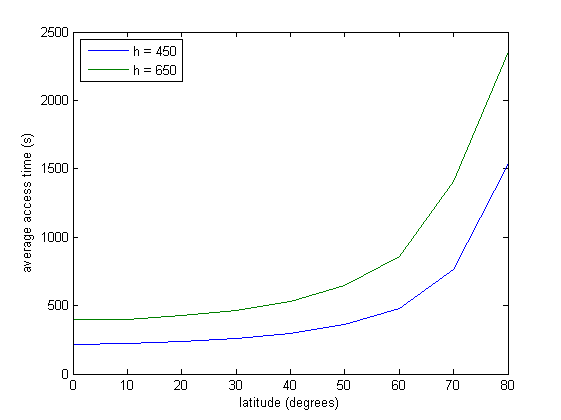
\includegraphics[width=1.0\textwidth]{Figures/accesstid450og650}
  \end{center}
  \caption[Accesstid for 450 og 650]{Access times for $h=450km$ and $h=650km$ as a function of ground station latitude}
  \label{fig:acctid}
\end{figure}

Since we don't know when the satellite will be launched we don't know the exact orbit. The project manager, Roger Birkeland, told us that we can assume the orbit will  have a height above the Earth somewhere between 450km and 650km and inclination of 98 degrees. The uncertainty in $h$ is critical, because the height above the earth dramatically changes the access time of a ground station, see Fig. \ref{fig:acctid}. 

\begin{figure}
  \begin{center}
    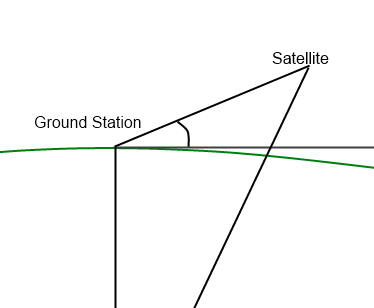
\includegraphics[width=0.7\textwidth]{Figures/groundstation_satelitte_geometry}
  \end{center}
  \caption[Ground station satellite geometry]{Illustration of geometry between a ground station and a satellite}
  \label{fig:gs_s_geom}
\end{figure}

The ground station can only communicate with a satelitte when it has a certain elevation. Which may depend on topology, atmosphere, antenna ...
In the following we assume that the minimum elevation is 25 degrees, maximum elevation is 90 degrees and no constraints on the azimuth angle.  For a illustration see Fig. \ref{fig:gs_s_geom}.

\begin{figure}
  \begin{center}
    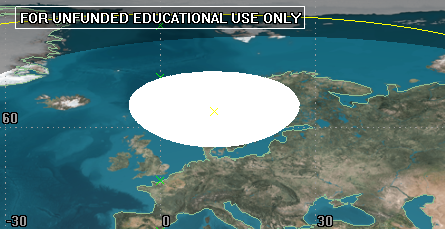
\includegraphics[width=0.8\textwidth]{Figures/ntnu_footprint}
  \end{center}
  \caption[ntnu footprint]{NTNU ground station range}
  \label{fig:ntnu_range}
\end{figure}

The result of this is that the ground station can communicate with the satelitte whenever the ground track is inside a rough circle centered on the ground station, see Fig. \ref{fig:ntnu_range} for the estimated "range" of the ground station at Gløshaugen operating with these constraints.

The Gløshaugen ground station will on average be able to communicate with the satellite 540 seconds per day if $h=450$ and 980 seconds per day if $h=650$. We don't know exactly how much data we need to download, but according to \cite{eks-kom} we'll need roughly 12 minutes (720 seconds) to download a single image. 

\subsection{Other ground stations}
Fig. \ref{fig:acctid} shows that the access time for a (near) polar satellite is nearly constant for ground stations at latitudes below 45 degrees. The access times of a ground station those low latitudes is in the 300 to 500 second range, i.e. about half a image, so we'll need about 2 ground stations at lower latitudes to download a single image. We may compare this to a single ground station located in Longyearbyen (78' N) which has a access time in the 1400 to 2300 second range, i.e. 2-3 images per day. 

\begin{figure}
  \begin{center}
    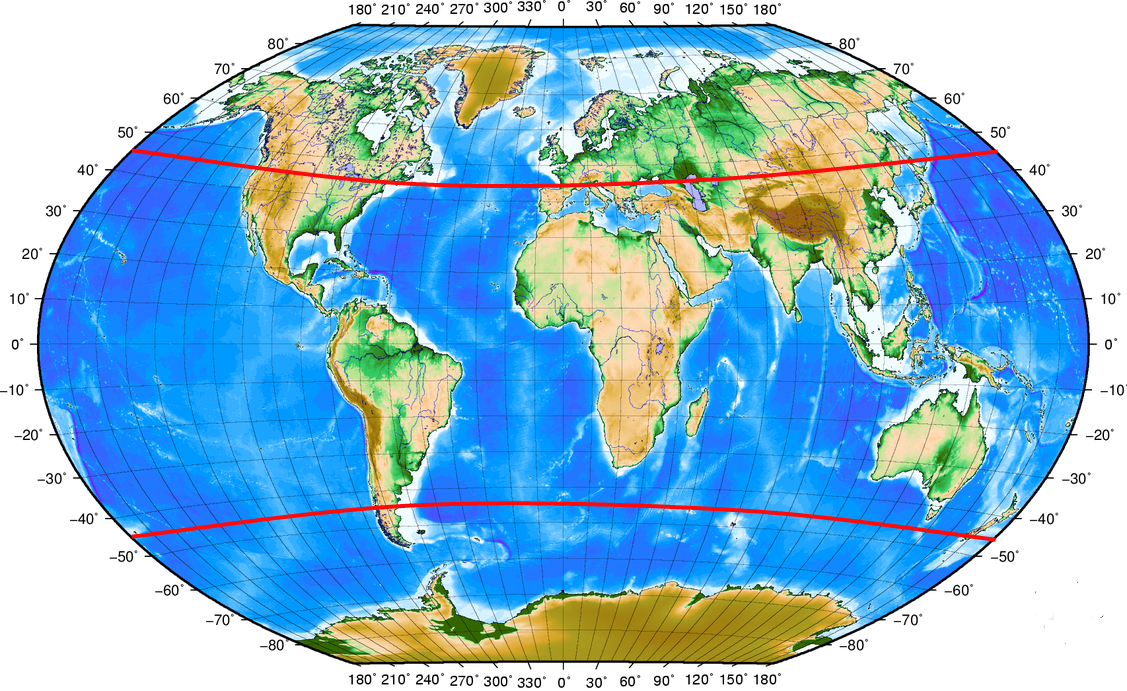
\includegraphics[width=0.9\textwidth]{Figures/verdenskart}
  \end{center}
  \caption[world]{Map of the World}
  \label{fig:world}
\end{figure}

Most prospective partners in this network are at lower latitudes (see Fig.  \ref{fig:world}). This means that to download 5 images through a network like this we need at least 8 other nodes in the network. Other stations will probably have some overlap with each other, down time, conflicting schedules etc. so the optimal number of nodes is probably far higher.




\section{Network technology for ground stations}
When we decided to work on a network of ground stations, we first looked into four different ground station network technologies. We first hoped to work on a BlueBox, but this would require support from Aalborg that we couldn't get, as they were busy with a satellite launch of their own. Because of this, we decided to look into Carpcomm, that seemed more complete and doable than connecting to PYXIS with a BlueBox.
\subsection{Genso}
information about Genso
\subsection{Carpcomm Space Network}
Carpcomm is a private company that delivers a plug and play ground station \cite{carpcomm-gs1} that costs \$700. The software for the ground station is open source and is provided pre.compiled for x86 and arm debian.
It is compatible with the Carpcomm Space Network \cite{carpcomm-sn}. 
The advantage of using this solution is that the network is actually functioning, though there are few other operational ground stations.
%\cite{carpcomm-gs1}
%\cite{carpcomm-sn}
\subsection{PYXIS}
The BlueBox is part of a distributed ground station network called PYXIS, developed primarily for the AAUSAT3 by Aalborg University (2013 \cite{aausat3}). The PYXIS goal is to offer a robust and effective ground station network for satellite developers, and one of the key factors is that everyone is free to setup a ground station using the open source BlueBox hardware. 

The PYXIS concept includes a backend server, BlueBox hardware and a Ground Station Server (GSS). The backend server runs an individual instance for each satellite utilizing the BlueBox, and is operated by the persons responsible for the ground station. 

The BlueBox itself is hardware to recieve and transmit signlas from the satellites.

Control of the BlueBox and ground station mechanics is handled by the GSS, and both the BlueBox and the GSS is operated by the responsible for the Ground station. 

Both the backend server and the GSS is already in place at each ground station, and to join the PYXIS network we would only have to make a BlueBox, and test that it works.

\section{Raspberry pi}
Raspberry Pi is a small computer, with everything gathered in one board. In our project we will be using the B model, revision 2, which have a 700MHz ARM CPU, 512MB of RAM and a SC-card reader, in addition to the leads to connect to different devices, for  the full overview, see figure \ref{fig:raspberrypihighlevel}. The recommended operating system is Raspbian, a linux distribution based on Debian. 

The Raspberry pi was originally intended to help teach programming, but it can also perform many of the standard computer tasks, and it can be connected to a monitor or tv using an HDMI lead. In our project we hope to be able to use a Raspberry pi to run the software required to control the ground stations. The software provided by the Carpcomm project has Raspbian as one of its supported platforms, so we hope this will work well.

\begin{figure}
	\begin{center}
		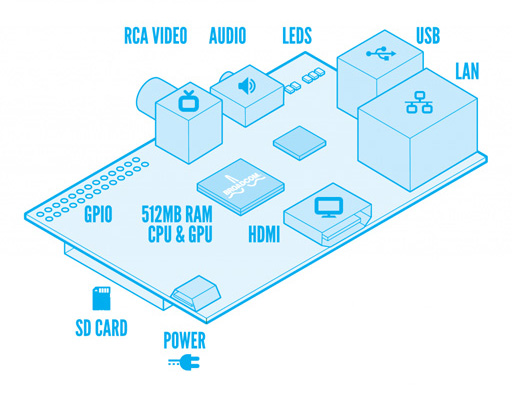
\includegraphics[width=0.7\textwidth]{Figures/raspberrypi_modelb_hl.jpg}
	\end{center}
	\caption[Raspberry pi highlevel]{A highlevel schemantic of the Raspberry pi, model B rev 2}
	\label{fig:raspberrypihighlevel}
\end{figure}

To control the movement of the antennas, an serial port is needed. Raspberry Pi has an serial port included in its gpio (general purpose input/output) connector. This serial port uses ttl-standard for its voltage levels, this is 0/3.3V while RS232 which is the standard used in computers uses (3V-15V)/-(3V-15V). Because of this an converter is needed. We chose to make an custom circuit board using the MAX3232 RS232 line driver. The circuit board is designed to be mounted on the gpio connector, because of small space in the case for the Raspberry Pi, the output is connected with cable to the external connector.

\begin{figure}
	\begin{center}
		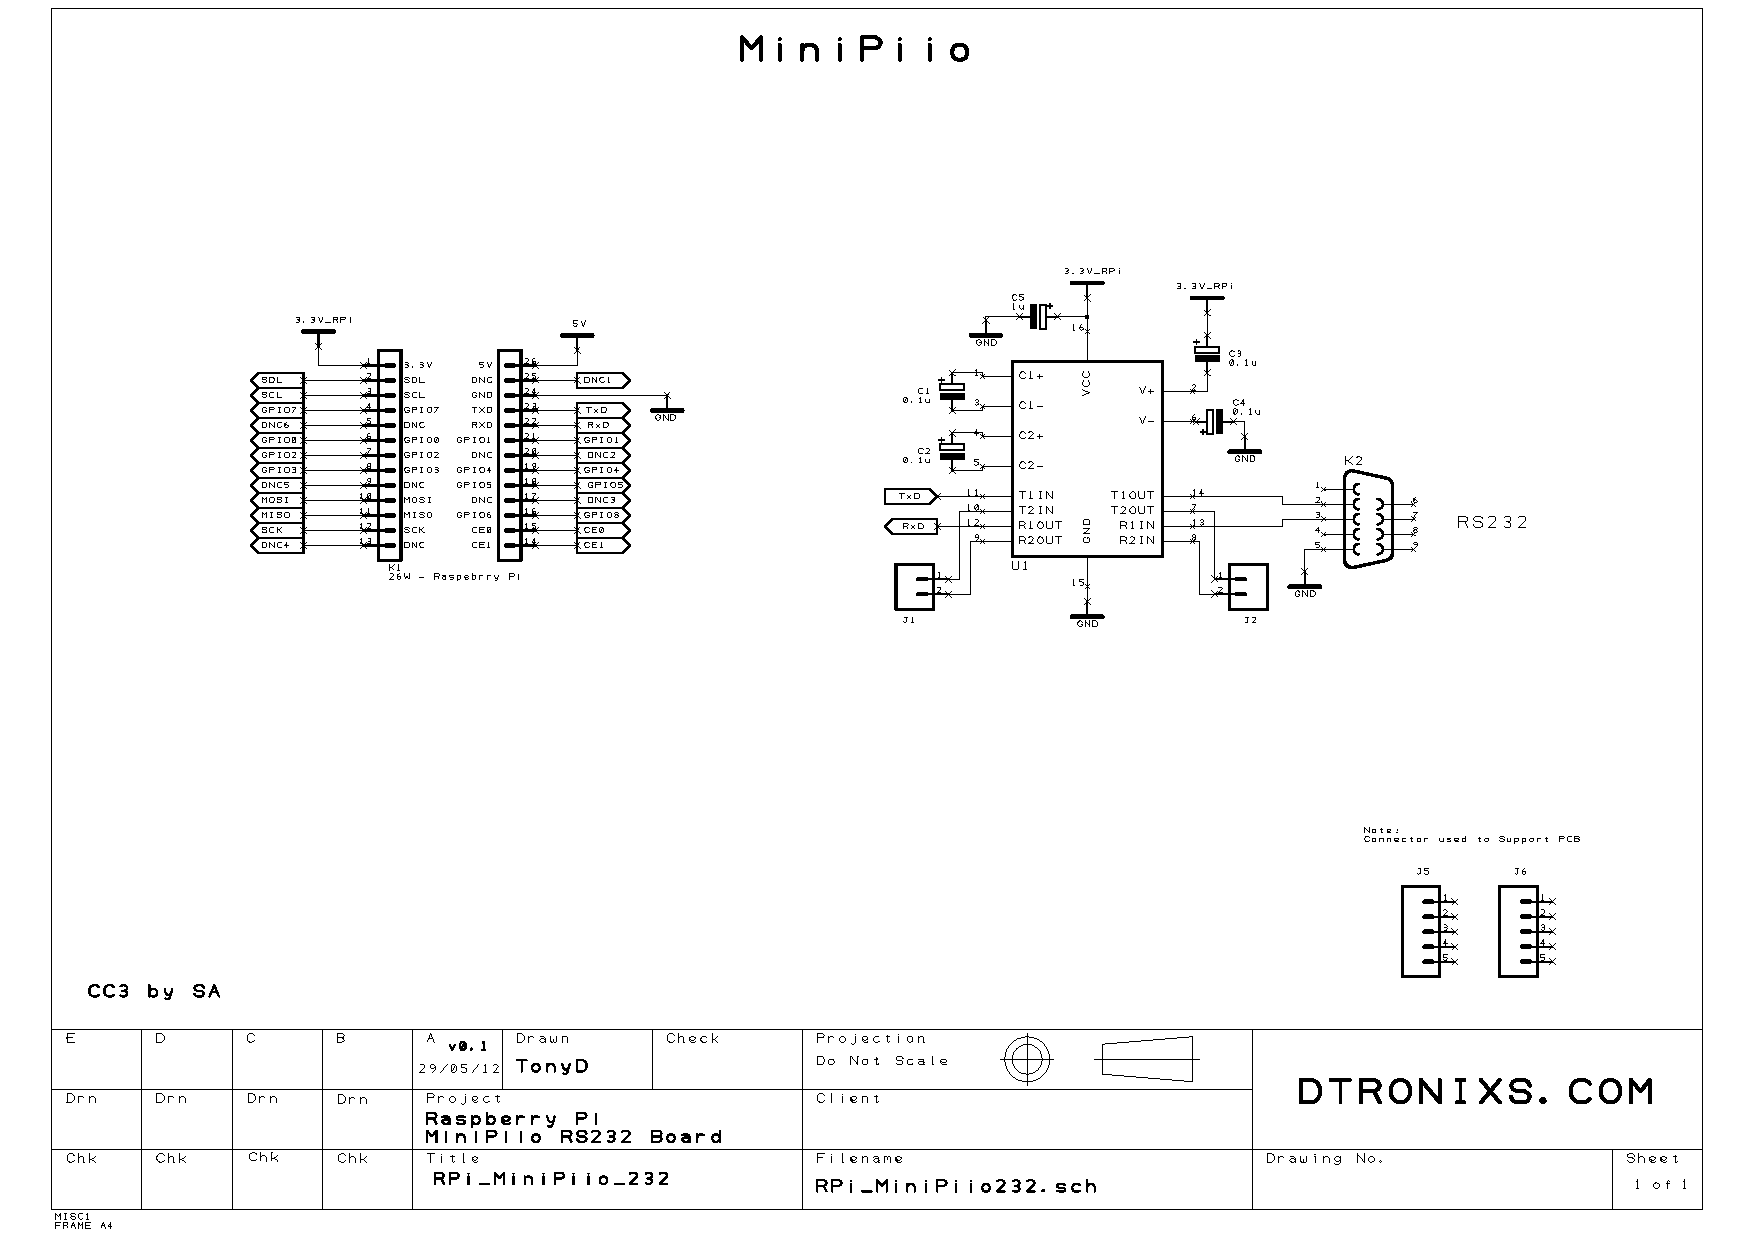
\includegraphics[width=0.7\textwidth, trim=400 250 100 100, clip=true]{../Schematics/UART-to-RS232.pdf}
	\end{center}
	\caption{Schematics for the RS232-converter}
	\label{fig:UART-RS232}
\end{figure}
\section{Solar Power}

Communication with the satellite through the groundstation network demands power from the satellite. Without any electrical power a satellite will not be able to support its payload or radio communication. NUTS double CubeSat uses sunlight as an energy source through solar panels. 

Solar panels base their operation on the ability to convert sunlight into electricity. By using semiconductors the photovoltaic effect can be exploited. The conversion process where the suns radiation is converted into an electrical current is achieved by creating mobile charged particles in the semiconductor. They are in turn separated by the device structure and produce the electrical current.(kilde) 

Batteries are used to store power during eclipse and support the payload. When the satellite is in eclipse the earth blocks the solar radiation and the battery must supply the power.

Identifying the satellites communication necessary to establish if a groundstation network is profitable. Forthcoming calculations are based on an estimate done by De Bruyne \cite{Satellite Power Systems}.

When estimating the period of the satellite the Earth and satellite orbit is assumed to be spheres. Kepler`s third law for circular orbits is used:

\begin{equation}
\left(\frac{2\pi}{T}\right)^2 = \frac{GM}{R^3}
\label{eq:Keplers_3}
\end{equation}

Where T is the period of the satellite, G is the gravitational constant\footnote{$G=\unitfrac[6.6742\cdot 10^{-11}]{km^3}{s^2}$}, M is the mass of the Earth\footnote{$M=\unit[5.9736\cdot 10^{24}]{kg}$} and R is the distance between the centers of mass of the Earth and the satellite.

\begin{equation}
T = 2\pi \left(\frac{R^3}{GM}\right)^{\frac{1}{2}}
\label{eq:satellite_period}
\end{equation}

where $R = R_\Earth + h$ where $R_\Earth$ is the radius of the earth\footnote{$R_\Earth = \unit[6371]{km}$} and h is the altitude of the satellite. 
Since it is uncertain what altitude the satellite will settle in after it is launched, two heights are used in the calculations and it's assumed that the satellite wil settle somewhere within interval $h_1=\unit[450]{km}$ and $h_2=\unit[650]{km}$. 
Which gives

\begin{equation}
T(h_1) = 5610s
\end{equation}

\begin{equation}
T(h_2) = 5850s
\end{equation}

when inserted into \autoref{eq:satellite_period}.

From De Bruyns equations \cite{Satellite Power Systems} the longest possible time in eclipse can be calculated. The worst case average power is approximately $P_{avg} = 5.42 W$ from by De Bryens calculations. This power is calculated when the satellite has its longest time in eclipse.

\begin{equation}
	t_{ecl,max} = 2R_{sat}\left(\frac{R_{sat}}{R\times M}\right)^{\frac{1}{2}}
	\label{Maximum time in eclipse}
\end{equation}

\begin{equation}
	P_{avg,orbit} = P_{avg}\times\frac{(t-t_{ecl,max})}{t}
	\label{Average effect during one orbit}
\end{equation}

Putting in $h_1 =\unit[450]{km}$ and $h_2 = \unit[650]{km}$ gives:

\begin{equation}
t_{ecl,max_1} = 2151.1 s = 35.9 min
\end{equation}

\begin{equation}
P_{avg,orbit_1} = 3.34W
\end{equation}

\begin{equation}
t_{ecl,max_2} = 2118.9 s = 35.3 min
\end{equation}

\begin{equation}
P_{avg,orbit_2} = 3.46W
\end{equation}

These are simplified calculations where the temperature changes of the solar cells is not taken into account. As the satellite moves through orbit the temperature will effect the solar cells, but including this effect requires more extensive calculations. The average power calculated here is based on worst-case estimate from De Bruyns \cite{Satellite Power Systems}, the real average power can be calculated with the exact orbit parameters. 

The battery used in the NUTS Cubsat wil consist of lithium-ferrite-phosphate cells $(LiFePO_4)$\cite{Overview of NUTS}. 
These cells have a typical voltage of 3.3 V. NUTS wil have $4\times \unit[1.1]{Ah}$ cells, where two is in serie and two is in parallel(parallell i serie eller serie i parallell?). This means a total of $C=\unit[2.2]{Ah}$ at $\unit[6.6]{V}$ (\cite{Satellite Power Systems} unødvendig?). This is used to calculate the worst-case Depth Of Discharge (DOD). The DOD represents the percentage of the discharged battery capacity expressed as a percentage of maximum capacity. It indicates the state of charge where $100\% $= empty and  $0\%$ = full (KILDE).

The battery capacity used during eclipse: 
\begin{equation}
C_{ecl} = \frac{P_{avg,orbit}}{V_tot}\times t_{ecl,max}
\label{Battery capacity}
\end{equation}

 \begin{equation}
DOD_{max} = \frac{C_{ecl}}{C_{tot}}
\label{Depth Of Discharge}
\end{equation}

Calculated with the different heights gives:

equation \ref{Battery capacity}
$C_{ecl_1} = \frac{3.34W}{6.6V}\times(\frac{35.9min}{60\frac{min}{hour}}) = 0.3Ah$

equation \ref{Depth Of Discharge}
$DOD_1 = 0.136 = 13.6 \%$

equation \ref{Battery capacity}
$C_{ecl_2} = \frac{3.46W}{6.6V}\times(\frac{35.3min}{60\frac{min}{hour}}) = 0.31 Ah$

equation \ref{Depth Of Discharge}
$DOD_2 = 0.141 = 14.1\%$

The battery capacity will decrease with the number of charge-discharge cycles. Discharge of at least 80\% is refered to as deep discharge. When the critical DOD is reached it will be in risk of battery failure. From our calcultations the DOD is not in the critical region. 

\vspace{5 mm}To establish the communication time a simplified power balance is used. 

\vspace{5 mm}$P_{radio} = 2.5 W$

$P_{payload} =$ $5 W$  in  $90s$

Microcontroller is in standby and with 18.5mA and 3.3V it uses:

$P_{standby} = 0.0612W$ 

These numbers are supplied from NUTS and are rough estimates of what can be expected.

\begin{equation}
P_{avg,orbit}\times t - P_{payload}\times 90 s - P_{standby}\times t= P_{radio}\times t_{communication}
\label{eq:communication_time}
\end{equation}

Inserting $h_1$ and $h_2$ into \autoref{eq:communication_time} gives:

\begin{equation}
t_{communication} = \unit[7172.12]{s} =\unit[110.5]{min}
\end{equation}

\begin{equation}
t_{communication} = \unit[7778.77]{s} =\unit[129.6]{min}
\end{equation}

The calculations on power- and orbit estimates results in long communication time. There are several simplifications done during this calculations that must be taken into account. The power drawn from the satellite are rough estimates and the available communication time will likely differ from the these results. The calculated communication time provides a good indication and it can be seen that it is time available to connected to a groundstation network.


